\documentclass[12pt,letterpaper]{article}
\usepackage[utf8]{inputenc}
\usepackage[spanish]{babel}
\usepackage{amsmath}
\usepackage{amsfonts}
\usepackage{amssymb}
\usepackage{graphicx}
\usepackage[left=2cm,right=2cm,top=2cm,bottom=2cm]{geometry}
\usepackage{pdfpages}
\usepackage{subfigure}
\author{}
\date{}

\begin{document}
%insertar portada
%\includepdf{figuras/Caratula}

\tableofcontents

%En este trabajo se explicará cómo realizar una presentación de un proyecto para los trabajos de laboratorio de la materia \textbf{Interfaces}.

\section{Introducci\'on}
En este trabajo se pretende desarrollar un tutorial que permita al usuario neófito poder iniciar sus primeros proyectos usando RTOS y comprender la arquitectura de los procesadores Cortex.\\
Este estudio aborda en primer lugar, las características principales de la placa y la correcta instalación del software que permite el desarrollo de códigos sobre ella; además se incluyen posibles problemas que puedan suceder en el proceso junto con sus soluciones.\\
Sobre el final de dicha sección se desarrolla una guía para la correcta configuración de el entorno gráfico, para poder ejecutar la compilación del primer ejemplo que nos indica que hemos finalizado satisfactoriamente la instalación del software de la EDU CIAA.\\
La siguiente sección comienza introduciendo al usuario en el uso de la placa a través de la biblioteca \textit{sAPI} (realizada por Eric Pernia) la cual nos permite el desarrollo de programas utilizando lenguaje C, nuestro propósito es brindar una explicación simple de la arquitectura de los procesadores Cortex y a su vez brindar una base para la siguiente sección del informe.\\
Sobre el inicio del siguiente apartado, se introduce al usuario sobre la programación a través de el sistema operativo \textit{OSEK OS}, el cual es el método de programación en el que se proyectó cuando se realizó el diseño de la placa. Nuestra meta es fijar las bases conceptuales principales de los sistemas operativos en tiempo real, e introducir al usuario a la programación de códigos simples y alentar al usuario a profundizar sobre este estudio.
%El informe técnico es una de las herramientas más valiosas que posee un profesional a la hora de poder comunicar sus ideas a otras personas. Es por esto que es necesario saber de qué forma se estructura un informe y cuáles son las pautas a seguir, de acuero a los usos y costumbres usados en diferentes tipos de publicaciones profesionales.

%Este documento describe cuales son las principales partes que componen un informe técnico. Además provee referencias a herramientas y publicaciones que ayudan a organizar mejor un informe, a usar en forma correcta las referencias bibliográficas y la correcta utilización del idioma castellano.

%Este modelo de informe está organizado como sigue: en la sección 2 se comenta sobre estilos, las partes que componen un informe técnico y las herramientas software para sistematizar su escritura. En la sección 3 se analizan los resultados usando distintas herramientas software y en la sección 4 se hacen las conclusiones.

\section{Desarrollo}
%Todo informe está compuesto por partes que están interrelacionadas. A su vez todo el informe está enmarcado en un estilo que hace al tipo de letra utilizado, tamaño de la letra, márgenes, etc.

\subsection{Origen del proyecto CIAA}
Sobre julio de 2013, la Secretaría de Planeamiento Estratégico Industrial del Ministerio de Industria de la Nación (SPEI) y la Secretaría de Políticas Universitarias del Ministerio de Educación de la Nación (SPU) convocaron a la Asociación Civil para la Investigación, Promoción y Desarrollo de los Sistemas Electrónicos Embebidos (ACSE) y a la Cámara de Industrias Electrónicas, Electromecánicas y Luminotécnicas (CADIEEL) a participar en el "Plan Estratégico Industrial 2020". A partir de dicha convocatoria se inició el desarrollo de la Computadora Industrial Abierta Argentina (CIAA).\\

El pedido inicial fue que desde el sector académico (ACSE) y desde el sector industrial (CADIEEL) se presenten propuestas para agregar valor en distintas ramas de la economía (maquinaria agrícola, bienes de capital, forestal, textil, alimentos, etc.) a través de la incorporación de sistemas electrónicos en procesos productivos y en productos de fabricación nacional. Debe destacarse que muchas empresas argentinas de diversos sectores productivos no incorporaban electrónica en sus procesos productivos o en sus productos, otras utilizaban sistemas electrónicos obsoletos, muchas utilizaban sistemas importados y sólo unas pocas utilizaban diseños propios basados en tecnologías vigentes y competitivas.\\

A partir de esta situación, la ACSE y CADIEEL propusieron desarrollar un sistema electrónico abierto de uso general, donde toda su documentación y el material para su fabricación estuviera libremente disponible en internet, con el objetivo de que dicho sistema pueda ser fabricado por la mayoría de las empresas PyMEs nacionales, y realizar modificaciónes en base a las necesidades específicas que puedan tener.

%Para hacer el informe se recomienda el uso de letra Times New Roman, tamaño 12, espaciado $ 1,5 $ entre líneas. Los títulos se pueden colocar en mayor tamaño y en negrilla. Las leyendas de tablas y figuras van en tamaño 12. Para las tablas la leyenda va justificada y para las figuras va centrada.

%Las figuras y las tablas deben estar numeradas y referenciadas dentro del texto que hace alusión a ellas. En la Fig. \ref{fig_Fig1} se puede observar una referencia a una figura y la figura referenciada.

%El tamaño de la hoja es A4, con márgenes de 2 cm. En algunos casos, como por ejemplo publicaciones en congresos se estila un estilo a dos columnas, como el que propone la IEEE\cite{A4_IEEE}. Este formato se puede descargar y es una plantilla en word o en latex que sirve de base.

%\begin{figure}[!t]
%\centering
%\subfigure[Referencia a una figura.]{\includegraphics[width=8 cm]{figuras/fig_01.jpg}}
%\subfigure[Figura referenciada.]{\includegraphics[width=8 cm]{figuras/fig_02.jpg}}
%\caption{Referencia a una figura.}
%\label{fig_Fig1}
%\end{figure}
Hoy en día la CIAA está disponible en la versión CIAA-NXP y otras seis versiones están en elaboración: CIAA-ATMEL, CIAA-FSL, CIAA-PIC, CIAA-RX, CIAA-ST, CIAA-TI. Además, se está trabajando en el firmware y en el software, para que la CIAA se pueda programar en lenguaje C utilizando una API especialmente diseñada para ser compatible con los estándares POSIX y que sea portable a diversos sistemas operativos de tiempo real.\\
Desde la concepción del proyecto, el diseño de la placa se encuentra pensada para soportar las condiciones hostiles de los ambientes industriales los que abundan ruidos, vibraciones, temperaturas extremas, picos de tensión e interferencias electromagnéticas, y además se diseñó de modo tal que pueda ser fabricada en Argentina.

\subsection{Descripción de la placa}


\begin{figure}[!h]
\centering
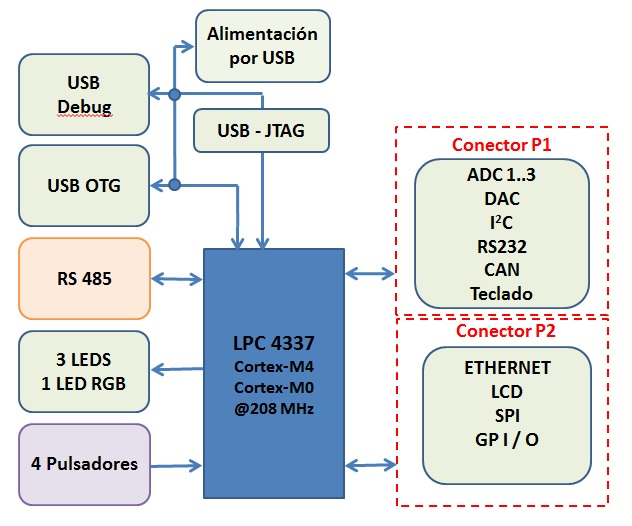
\includegraphics[width=8 cm]{figuras/diagramaenbloques.jpg}
\caption{Diagrama en bloques de EDU CIAA basado en LPC4337.}
\label{Fig1}
\end{figure}



La CIAA es una plaqueta electrónica provista de un microcontrolador y puertos de entrada y salida, cuyo diseño se encuentra disponible en Internet, dicha placa fue concebida para ser utilizada para sistemas de control de procesos productivos, agroindustria, automatización, entre otras; es notable destacar que gracias a la posibilidad del acceso a la información de dicha plataforma, cualquier empresa que desee utilizarla para la elaboración de sus productos puede rediseñarla; de modo que esto fomenta el diseño y la fabricación nacional de sistemas electrónicos.\\

\begin{figure}[!h]
\centering
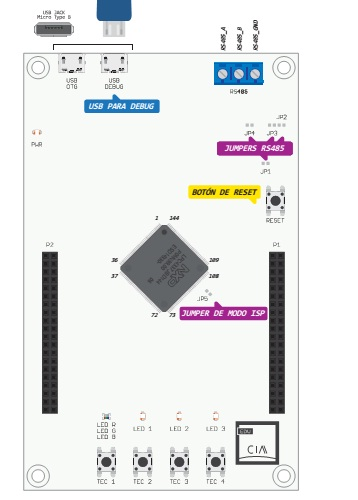
\includegraphics[width=8 cm]{figuras/FIGURA_1.jpg}\\
\caption{Imagen frontal de placa}
\label{Fig2}
\end{figure}

La placa EDU CIAA es la versión educativa de esta,la cual se encuentra diseñada con el propósito de conseguir una plataforma base para el desarrollo de proyectos educativos, en este caso, se busca proporcionar las bases del desarrollo de códigos utilizando RTOS.\\

%%

Sobre la Figura 1 \ref{Fig1} se proporciona el diagrama en bloques de la placa, puede observarse que la placa cuenta con 2 puertos micro-USB (uno para aplicaciones y debugging, otro para alimentación); 4 salidas digitales implementadas con leds RGB, 4 entradas digitales con pulsadores; 1 puerto de comunicaciones RS485 con bornera. La Figura 2 \ref{Fig2} nos muestra  una imagen frontal de la placa; nótese la presencia de dos puertos sobre los cuales se ubican los pines correspondientes a la placa, la Figura 3 \ref{Fig3} ilustra el distribución de dichos pines sobre cada puerto.

%%

Sobre el puerto P1, se ubican los siguientes módulos:

\begin{enumerate}
\item 3 entradas analógicas ($ADC0_ 1,2 y 3$)
\item 1 salida analógica (DAC0).
\item 1 puerto I2C.
\item 1 puerto asincrónico full duplex (para RS-232).
\item 1 puerto CAN.
\item 1 conexión para un teclado 3x4.
\end{enumerate}

Sobre el puerto P1, se ubican los siguientes módulos:

\begin{enumerate}
\item 1 puerto Ethernet
\item 1 puerto SPI
\item 1 puerto para Display LCD con 4 bits de datos, Enable y RS.
\item pines genéricos de I/0.
\end{enumerate}

\section{Instalacion de Software}

\subsection{Conceptos previos}
El desarrollo de codigos para sistemas embebidos tiene ciertas semejanzas con el desarrollo de aplicaciones en las PC, en nuestro caso particular se utiliza un compilador llamado \textit{GCC} con soporte para la compilación de proyectos sobre los procesadores basados en la arquitectura ARM, en este caso particular, el compilador utilizado para el procesador de la EDU CIAA (el cual es el LPC4337) se lo denomina \textit{arm-none-eabi-gcc}.\\

Para la ejecución de la depuración de algun programa previamente compilado, el hardware de la CIAA viene provisto con el chip \textit{FT2232H}, que se encarga de hacer un puente entre la interfase JTAG del microcontrolador, y el USB que conecta a la PC en el puerto USB dedicado al debug. Mediante la herramienta de código abierto \textit{OpenOCD (On Chip Debugger)} se controla el chip \textit{FT2232H} por el USB y ademas todo lo referido al JTAG. Luego la herramienta de depuración \textit{GDB} utilizado en el IDE-Eclipse que se instala, se comunica sobre el puerto 3333 (TCP) que el \textit{Open OCD} tiene en escucha esperando la conexión.\\

Debe tenerse en cuenta que el chip \textit{FT2232H} posee 2 canales de comunicación independientes (A y B), sin embargo, ambos salen por el mismo USB, de modo que la PC detecta 2 dispositivos distintos (en realidad es uno compuesto). Uno de ellos, se conecta al JTAG manejado por \textit{OpenOCD} como fue mencionado, mientras que el otro se ve como un puerto virtual COM. Este último sirve principalmente para la depuración.\\
%%CONSIDERAR SI CIERTA PARTE VA A IR A SECCION INSTALACION
Dado que al funcionará como dos dispositivos distintos, para cada uno de ellos debe realizarse la instalación de un driver adecuado, en principio debe optarse por realizar la instalación de los drivers por defecto del fabricante FTDI para puerto virtual.\\ %Considerar%

\subsection{Firmware de la EDU CIAA}
Considerando que el usuario previamente ha trabajado sobre placas de desarrollo tales como la MCE Debug, etc, y sobre microcontroladores PIC. Es necesario destacar un concepto teórico que nos brinda la posibilidad de fundamentar el trabajo sobre la placa EDU CIAA. Al trabajar sobre los otros dispositivos, es común la utilización de programas tales como \textit{MPLABX}, o \textit{PICC} a través del compilador \textit{CCS Compiler}; puntualmente; cuando se inicia un nuevo proyecto a traves de la herramienta de creación de la misma, es usual configurar este proyecto de manera que el software IDE genera un archivo \textit{makefile} para la compilación del proyecto.\\
En este caso particular, el software IDE de la EDU CIAA trabaja de forma ligeramente distinta, el usuario debe crear un archivo \textit{makefile} (basándose en un archivo proporcionado previamente, denominado \textit{Makefile.config}) para poder efectuar la compilación del archivo y lograr la correcta configuración del programa, sobre la placa EDU CIAA. Dentro de dicho archivo se establece la configuracion para la arquitectura del procesador utilizado.
%%CONSIDERAR POSICION DEL SIGUIENTE PARRAFO%%
Cuando se desea realizar el primer proyecto sobre la placa, el usuario debe crear su propio archivo \textit{Makefile.mine}, de manera que ésta se encuentra basada en el archivo \textit{Makefile.config} brindado previamente al momento de establecer un nuevo proyecto añadiendo un Firmware que previamente ha sido diseñado por los creadores de la placa.\\
Debe tenerse en cuenta que la dinámica de trabajo sobre la placa se encuentra pensada para trabajar sobre la plataforma de versionado \textit{Git}; en este caso en particular, el archivo \textit{Makefile.mine} se encuentra diseñado de forma tal que dicho archivo sea ignorado al sincronizar su repositorio local, con su repositorio remoto (ubicado sobre \textit{Github}).\\
En el Makefile.mine se pueden editar y configurar los siguientes parámetros:
\begin{enumerate}
\item \textbf{ARCH}  indica la arquitectura del hardware para la cual se desea compilar. Ej: x86, cortexM4.
\item \textbf{CPUTYPE} indica el tipo de CPU. Ej: none, ia32, ia64, lpc43xx.
\item \textbf{CPU} indica la CPU para la que se desea compilar. Ej: none, lpc4337.
\item \textbf{COMPILER }es el compilador a utilizar. Ej: gcc.
\item \textbf{BOARD }es la placa sobre la cual se trabajaca (CIAA-NXP, EDU-CIAA-NXP, etc.)
\item \textbf{PROJECT }es el Path al proyecto a compilar. Ej: examples$\$(DS)blinking_base$.
\end{enumerate}
Se utiliza la variable \$(DS) para indicar el separador de directorios (de manera automática se usa '/' para linux y '\' para windows).\\

En el mismo Makefile aparecen al comienzo comentarios donde se indican los valores que pueden tomar estos parámetros.\\

Otro concepto importante sobre el cual se tiene en cuenta cuando se desarrollan proyectos propios, es que cada proyecto tiene también su propio archivo \textit{Makefile}.El mismo se encuentra bajo el directorio\textbf{mak} en el directorio principal del proyecto o ejemplo. En el ejemplo \textbf{examples/blinking} el makefile del ejemplo se encuentra en \textbf{examples/blinking/mak} y se llama \textbf{Makefile}.\\

Sobre este \textit{Makefile} contiene las siguientes definiciones:

\begin{enumerate}
\item \textbf{project} el nombre del proyecto y por ende nombre del ejecutable.
\item \textbf{\$(project)\_PATH} es el directorio del proyecto.
\item \textbf{INCLUDE} los paths a indicar al compilador para buscar includes files.
\item \textbf{SRC\_ FILES} archivos a compilar ya sean archivos c como c++.
\item \textbf{OIL\_ FILES} configuración del sistema operativo (si es utilizado).
\end{enumerate}

Cada proyecto incluye en su Makefile los módulos (aca digo que son los módulos) a compilar en una variable llamada MODS, por ejemplo:\\
------------------------decidir si poner como imagen o como texto\\
MODS += modules$\$(DS)posix$ \
        modules$\$(DS)ciaak $\
        modules$\$(DS)config$ \
        modules$\$(DS)bsp $\
        modules$\$(DS)platforms$\\

Es recomendable utilizar \$(DS) en vez de / o \ para mantener la compatibilidad entre sistemas operativos (Linux, Windows, MAC OS).
{
\subsection{Estructura de Directorios de Firmware de EDU CIAA}
En el directorio principal luego de hacer un git clone o al bajar una release oficial se pueden encontrar los siguientes Directorios y Archivos:


\begin{figure}[!h]
\centering
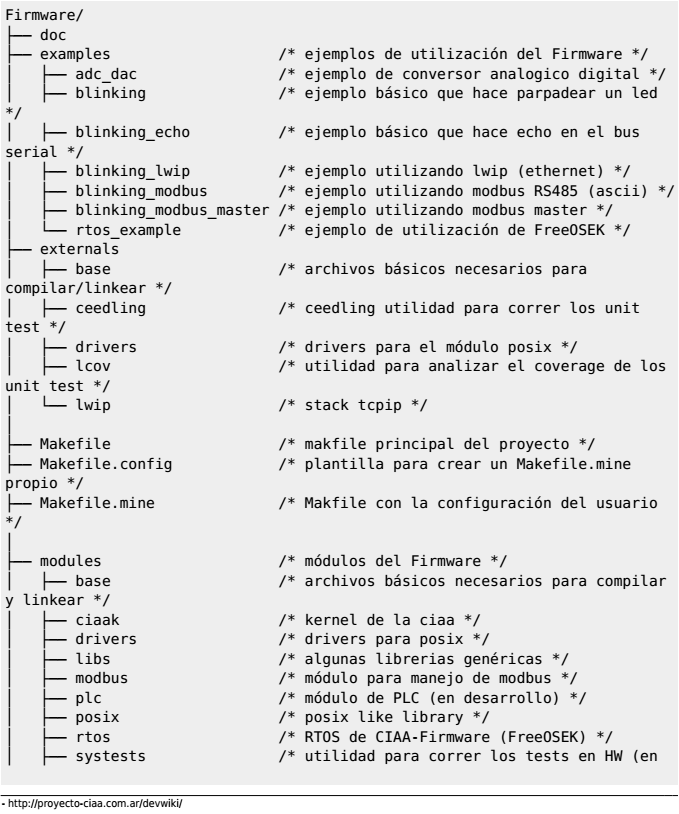
\includegraphics[width=8 cm]{figuras/est_directorios_ciaa.png}\\
\caption{Estructura de directorios del Firmware}
\label{Fig3}
\end{figure}

\textbf{Directorio $"externals"$(Software y Tools Externos)}\\
Este directorio contiene el Software y Tools externos al CIAA-Firmware, que son necesarios para compilar, testear, etc. el Firmware. Tenga en cuenta que el Software y Tools en esta carpeta no son parte de CIAA-Firmware y pueden contener otras licencias. Sobre la \ref{Tab1} se ilustra los contenidos del directorio y su descripción.

\begin{table}
\begin{center}
\begin{tabular}{|l|l|}
\hline\hline
ceedling & Tool utilizada para los Unit Tests o Pruebas Unitarias\\ \hline
base & Fuentes, headers y linker scripts necesarios para poder compilar y linkear el código en la plataforma\\ \hline
drivers & Drivers provistos por el proveedor del chip, los cuales son luego adaptados al formato de la CIAA.\\ \hline
\end{tabular}
\caption{Tabla1}
\label{Tab1}
\end{center}
\end{table}

\textbf{modules (out (Archivos de salida)}\\
La \ref{Tab2} contiene todos los archivos generados por el CIAA-Firmware:\\

\begin{table}[h]
\begin{center}
\begin{tabular}{|l|l|}
\hline\hline
bin & Contiene el binario del proyecto, es el archivo que se va a correr en la PC o a cargar en el CIAA-Firmware\\ \hline
gen & Archivos generados de OSEK RTOS\\ \hline
lib & Por cada Módulo el make genera un archivo .a, osea una libreria\\ \hline
obj & Todos los archivos fuentes son compilados a object files y almacenados en este directorio\\ \hline
\end{tabular}
\caption{Tabla 2}
\label{Tab2}
\end{center}
\end{table}

}
\subsection{Iniciación a través de ejemplos}
Sobre el Firmware de la placa se distribuyen varios ejemplos los cuales se encuentran en la carpeta \textbf{examples} y pueden ser utilizados como base para iniciar cualquier proyecto.
Cualquiera de los ejemplos puede ser copiado y utilizado de base para nuevos proyectos. Por ejemplo con el siguiente comando:	\textit{cp -r $examples/blinking projects/my\_proyect$}\\
Y adaptando el Makefile.mine indicado: $PROJECT_PATH = projects/my\_project$.
%Un informe debe dividirse en partes para la correcta explicación del proyecto que se quiera divulgar. Estas partes son:
%\begin{enumerate}
 %\item \textbf{Portada o carátula}: esta es la primera página y en ella debe estar:
 %\begin{itemize}
 %	\item Escudos de la institución en donde se realiza la actividad
 %	\item Nombre de la materia.
 %	\item Si es un trabajo final de materia o si es un proyeto de laboratorio.
 %	\item Título del trabajo que resuma en forma clara y concisa la idea principal del proyecto.
 %	\item Nombre y apellido de los autores.
 %	\item Año
 %\end{itemize}
% El diseño de la carátula es libre, pero es recomendable que sea agradable y armoniosa.
% 	\item \textbf{Introducción}. Describe en qué consiste el proyecto que se ha desarrollado, las partes que lo componen y si se ha logrado el objetivo. Se comenta, además, sobre la bibliografía que se utilizó para su desarrollo y cómo está organizado el informe.
% 	\item \textbf{Desarrollo}: Esta etapa describe el diseño en sí del proyecto, comentando cada parte en forma detallada. Esta sección puede tener varias subsecciones para que sea más claro y ordenado el informe, como por ejemplo, el desarrollo del software, el desarrollo del hardware, el acondicionamiento de una señal de un sensor, el funcionamiento de un sensor en particular, etc.
% 	\item \textbf{Resultados}: En esta sección se muestran los datos o resultados obtenidos, capturas de osciloscopios. Se comenta sobre los datos obtenidos y si se ha logrado el objetivo buscado en el proyecto.
% 	\item \textbf{Conclusiones}: Presenta la evaluación e interpretación de los resultados obtenidos, los inconvenientes que se han encontrado durante el desarrollo del proyecto y posibles propuestas de mejoras en el caso de que los resultados pudieran ser obtenidos u optimizados con otros métodos a los aplicados.
% 	\item \textbf{Referencias}: En esta parte van todas la fuentes de información que se han utilizado en el proyecto, como por ejemplo, bibliografía, páginas web, apuntes de la cátedra o apuntes de otras universidades. La forma de referenciar es como se detalla en este instructivo.
 %	\item \textbf{Apéndices}: Pueden ser útiles en el caso de que la descripción detallada de un material pueda distraer del texto de trabajo. Aquí se puede incluir el código de un programa o la descripción del uso de una herramienta.
%\end{enumerate}

\subsection{Software para realizar informes}

%En la actualidad existen muchos programas para realizar un informe que ayudan a que la tarea sea más sencilla, en el especial en la numeración de tablas, fórmulas y figuras, como así también en la numeración de capítulos, secciones, subsecciones, etc.

%Entre estas herramientas de software se puede encontrar:
%\begin{itemize}
%	\item \textbf{TexMaker\cite{texmaker}}: es un editor gratuito multiplataforma distribuido bajo la licencia GPL para escribir documentos de texto, que integra muchas herramientas necesarias para desarrollar documentos con LaTeX en una sola aplicación. Texmaker incluye soporte Unicode, corrección ortográfica, auto-completado, plegado de código y un visor incorporado en pdf con soporte de synctex y el modo de visualización continua.
%	\item \textbf{Lyxs\cite{Lyx}}: es un programa gráfico multiplataforma creado por Matthias Ettrich que permite la edición de texto usando LaTeX, por lo que «hereda» todas sus capacidades (notación científica, edición de ecuaciones, creación de índices, etcétera). Se trata de un procesador de textos en el que el usuario no necesita pensar en el formato final de su trabajo, sino sólo en el contenido y su estructura (WYSIWYM) (Lo Que Ves Es Lo Que Quieres Decir, por sus siglas en Inglés), por lo que puede ser utilizado para editar documentos grandes (libros) o con formato riguroso (tesis, artículos para revistas científicas), con facilidad.
%	\item \textbf{Microsoft Word \cite{office}}: es una aplicación informática orientada al procesamiento de textos. Fue creado por la empresa Microsoft, y viene integrado en el paquete ofimático denominado Microsoft Office. Originalmente fue desarrollado por Richard Brodie para el computador de IBM bajo sistema operativo DOS en 1983. Versiones subsecuentes fueron programadas para muchas otras plataformas, incluyendo, las computadoras IBM que corrían en sistema MS-DOS (1983). Es un componente de la suite ofimática Microsoft Office; también es vendido de forma independiente e incluido en la Suite de Microsoft Works. Las versiones actuales son Microsoft Office Word 2013 para Windows y Microsoft Office Word 2011 para Mac. Actualmente es el procesador de texto más popular del mundo. No está orientado a la edición de textos científicos por lo que a la larga se hace más complicado su uso.
%\end{itemize}

%\section{Recomendaciones}
%Es necesario tener claro que es lo que se desea comunicar y ordenarlo antes de comenzar a escribir. Para esto sirve ir escribiendo en un borrador los pasos que se van cumpliendo mientras se va realizando el proyecto. Una vez terminado el proyecto, es decir, que está funcionando de acuerdo a los requerimientos planteado, se hacen las capturas de pantalla de la PC y del osciloscopio necesarias. 

%Luego se definen las secciones que formarán parte del informe; es aconsejable que el nombre haga referencia a lo que la sección trata, como así también el nombre de las subsecciones. Hay nombres de secciones que no se pueden cambiar como por ejemplo \textbf{Introducción}, \textbf{Resultados}, \textbf{Conclusiones}. Si es necesario agregar nuevas secciones o cambiarles el título en función de cómo se vaya desarrollando el trabajo \cite{Informe}.

%Es conveniete tener una librería de distintos formatos de informes y usarlos como plantillas. Esto permite tener siempre una estructura base y solamente dedicarse a escribir.

\section{Conclusiones}
%Es importante tener práctica en el desarrollo de informes y presentación de trabajos de desarrollo e investigación. Agiliza la creación de informes, ayuda a ordenar las ideas que se desean explicar, y permite hacer llegar de forma clara el trabajo desarrollado a muchas personas.

\begin{thebibliography}{99}
%\bibitem{A4_IEEE} http://www.ieee.org/conferences\_events/conferences/publishing/templates.html
%\bibitem{texmaker} http://www.xm1math.net/texmaker/
%\bibitem{Lyx} http://www.lyx.org/
%\bibitem{office} https://www.microsoft.com/es-ar/
%\bibitem{Informe} \textit{Cómo escribir un paper. Orientaciones y consejos}. Pedro Barrientos Loayza. Septiembre de 2012.
%\bibitem{guia} \textit{Informes Técnicos - Guía de redacción y presentación}. Pablo D. Ronco. FIUBA. Agosto 2011. 
\end{thebibliography}

\end{document}
